\documentclass{beamer}
\usepackage[utf8]{inputenc}
\usepackage[spanish]{babel}
\usepackage{graphicx}
\usepackage{amsmath} % Para notación matemática
\usepackage{adjustbox} % Para ajustar el tamaño de tablas
\usepackage{lipsum} % Para texto de prueba
\usepackage{changepage} % Para ajustar márgenes temporalmente
\usepackage{booktabs} %

\title{Buscando caminos de sofisticación: Complejidad económica y cambio estructural del Ecuador}
\author{David Escandón \\ Universidad de la República \\ Tesis de Maestría en Economía \\ Tutora: Flavia Rovira}
\date{Diciembre 2024}

\begin{document}

% Portada
\begin{frame}
    \titlepage
\end{frame}

% Resumen
\begin{frame}{Resumen}
    \begin{itemize}
        \item \textbf{¿Qué se hace?} Se identifican bienes y mercados que podrían contribuir a mayor sofisticación de la capacidad exportadora del país.
        \item \textbf{¿Cómo se hace?}
        \begin{itemize}
            \item Selección de productos a través de un esquema de pesos sobre medidas de complejidad y distancia.
            \item Cálculo de medidas de potencial implementando un modelo de gravedad.
        \end{itemize}
        \item \textbf{¿Qué se encuentra?} Bienes que el país no incorpora significativamente en su política industrial y mercados potenciales para estos bienes.
    \end{itemize}
\end{frame}

% Motivaciones: Contexto histórico
\begin{frame}{Motivaciones: Contexto histórico y actual del Ecuador}
    \begin{itemize}
        \item Dependencia histórica del petróleo desde los años setenta.
        \item Economía dolarizada desde el año 2000.
        \item Durante el boom petrolero (2004-2017), el país logró crecimiento económico mediante estímulos públicos.
        \item Problemas actuales: déficit fiscal, endeudamiento y dependencia de recursos externos.
    \end{itemize}
\end{frame}

% Motivaciones: Teorías de desarrollo
\begin{frame}{Motivaciones: Teorías de desarrollo}
    \begin{itemize}
        \item Las naciones desarrolladas son más diversificadas.
        \item El crecimiento económico está vinculado a la especialización exportadora (Imbs y Wacziarg, 2003).
        \item Las exportaciones reflejan capacidades como know-how colectivo y sofisticación económica.
    \end{itemize}
\end{frame}

% Datos
\begin{frame}{Datos}
    \begin{itemize}
        \item Fuentes principales: COMTRADE, Banco Mundial, CEPII.
        \item Período analizado: 1995-2019.
        \item Limpieza de bienes y países según exportaciones.
        \item Resultados:
        \begin{itemize}
            \item 1,214 bienes clasificados en el sistema armonizado (HS).
            \item 28,259,010 observaciones para medidas de potencial.
        \end{itemize}
    \end{itemize}
\end{frame}

% Estrategias de Selección

% Estrategias de Selección
\begin{frame}{Estrategias de Selección: Matrices de Especialización}
    \begin{itemize}
        \item Matriz de especialización: Ventajas comparativas Reveladas ($VCR_{c,p,t}$).
        \begin{equation} 
      VCR_{c,p,t} = \frac{\frac{Xval_{c,p,t}}{\sum_{c}Xval_{c,p,t}}}{\frac{\sum_{p}Xval_{c,p,t}}{\sum_{cp}Xval_{c,p,t}}}
    \end{equation}
        \item Matriz de especialización binaria ($M_{c,p,t}$). 
    \end{itemize}
    \\
    \begin{equation}
    \fontsize{8}{10}\selectfont
    M_{c,p,t} =
    \begin{cases}
    1 & \text{si } \left( \frac{1}{3} \sum_{i=0}^{2} VCR_{c,p,t-i} \right) > 1 \ \text{o } \left( \frac{1}{4} \sum_{i=0}^{3} VCR_{c,p,t-i} \right) > 1, \\
    0 & \text{lo contrario}.
    \end{cases}
    \tag{2}\label{eq:mcpt}
    \end{equation}
    \vspace{-0.5cm}
\end{frame}

% Estrategias de Selección: Espacio de producto y Proximidad
\begin{frame}{Estrategias de Selección: Espacio de producto y Proximidad}
    \begin{itemize}
        \item En el espacio de producto, cada nodo representa un producto y cada enlace ponderado mide la proximidad entre dos productos.
        \item La proximidad está calculada basado en una simple idea: si un país exporta determinados productos, es más probable que pueda exportar nuevos productos que estén relacionados a los que ya se encuentra exportando.
    \end{itemize}
    \[
    \varphi_{p,p'} = \frac{\sum_{c}M_{c,p}M_{c,p'}}{\max(k_{p,0}k_{p',0})}
    \]
    \begin{center}
        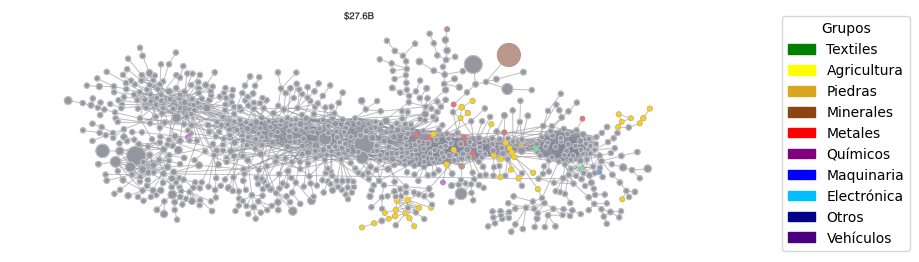
\includegraphics[width=0.8\textwidth]{Figura14.png}
    \end{center}
\end{frame}

% Matriz de países y productos
\begin{frame}{Matriz de países y productos}
    \begin{table}[h!]
    \centering
    \begin{tabular}{c|cccc|c}
        \hline
        \textbf{País / Producto} & \textbf{p1} & \textbf{p2} & \textbf{p3} & \textbf{...} & \textbf{Diversidad} \\
        \hline
        \textbf{c1} & 1 & 0 & 1 & ... & $D_1$ \\
        \textbf{c2} & 0 & 1 & 1 & ... & $D_2$ \\
        \textbf{c3} & 1 & 1 & 0 & ... & $D_3$ \\
        \textbf{...} & ... & ... & ... & ... & ... \\
        \textbf{cN} & 0 & 1 & 1 & ... & $D_N$ \\
        \hline
        \textbf{Ubicuidad} & $U_1$ & $U_2$ & $U_3$ & ... &  \\
        \hline
    \end{tabular}
    \end{table}
\end{frame}

\begin{frame}{Estrategias de Selección: Medidas de Complejidad}
    \begin{itemize}
        \item Índice de complejidad económica (ECI).
        \[
        k_{c,N} = \frac{1}{k_{c,0}} \sum_{p} M_{c,p} \cdot k_{p,N-1}

        \]
        \item Índice de complejidad de producto (PCI).
        \[
        k_{p,N} = \frac{1}{k_{p,0}} \sum_{c} M_{c,p} \cdot k_{c,N-1}
        \]
        \item Basados en el método iterativo de Hidalgo y Hausmann (2009).
    \end{itemize}
\end{frame}
%\begin{frame}{Estrategias de Selección: Distancia y OGI}
 %   \begin{itemize}
  %      \item Distancia.
   %     \item Índice de Oportunidad de Ganancia (OGI).

    %\end{itemize}
%\end{frame}

% Estrategias de Selección: Distancia y OGI
\begin{frame}{Estrategias de Selección: Distancia y OGI}
    \begin{itemize}
        \item \textbf{Distancia:}
        \begin{equation} \tag{13}
        d_{c,p} = \frac{\sum_{p'} (1 - M_{c,p'}) \varphi_{p,p'}}{\sum_{p'} \varphi_{p,p'}} \quad \text{; } 0 \leq d_{c,p} \leq 1
        \end{equation}

        \item \textbf{Índice de Oportunidad de Ganancia (OGI):}
        \begin{equation} \tag{15}
        OGI_{cp} = \left[\sum_{p'}\frac{\varphi_{p,p'}}{\sum_{p''}\varphi_{p'',p'}}(1-M_{cp'})PCI_{p'} \right]
        \end{equation}
    \end{itemize}
\end{frame}

% Estrategias de Selección: Problemática
\begin{frame}{Estrategias de Selección: Problemática}

    \begin{center}
        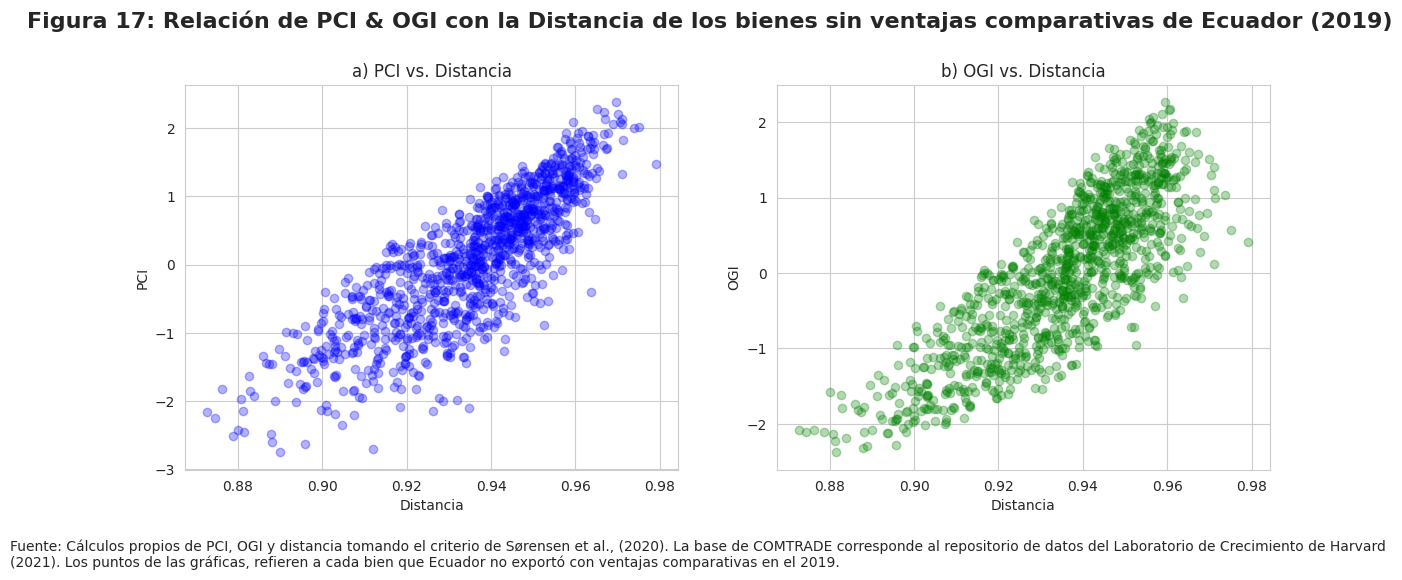
\includegraphics[width=1.05\textwidth]{Figura17.png}
    \end{center}
\end{frame}

% Estrategia de selección: "Esquema de pesos"
\begin{frame}{Esquema de asignación de pesos}
    \begin{table}[!ht]
    \centering
    \begin{adjustbox}{max width=0.9\textwidth}
    \begin{tabular}{cccccccc}
    \multicolumn{1}{l}{Tabla 3: Esquema de estrategias} & & & & & & & \\
    \hline
    \\
    \textbf{Estrategia} & \textbf{Componente} & ~ & \textbf{Ponderación} & ~ & ~ & ~ & ~ \\ 
    \hline\\
    ~ & ~ & Distancia & PCI & OGI & ~ & ~ & \\
    Apalancamiento \& Soporte & Frutas de Rápido Alcance & 0.45 & 0.25 & 0.30 & ~ & ~ & \\
    (0.1\textless VCR \textless1) & Apuestas Estratégicas & 0.20 & 0.20 & 0.60 & ~ & ~ & ~ & ~ & ~ \\ 
    Diversificar \& Escalar & Frutas de Rápido Alcance & 0.65 & 0.15 & 0.20 & ~ & ~ &  \\ 
    (VCR\textless0.1) & Apuestas Estratégicas & 0.50 & 0.10 & 0.40 & ~ & ~ & ~ & ~ & ~ \\ 
    \hline
    \end{tabular}
    \end{adjustbox}
    \caption*{Fuente: Esquema de ponderación tomado de la propuesta de Sørensen et al. (2020).}
    \end{table}
\end{frame}

% Estrategias de Selección: Resultados
\begin{frame}{Estrategias de Selección: Resultados}
    \begin{itemize}
        \item 79 bienes en total: 41 de Apalancamiento y Soporte y 38 de Diversificar y Escalar.
    \end{itemize}
    \begin{center}
        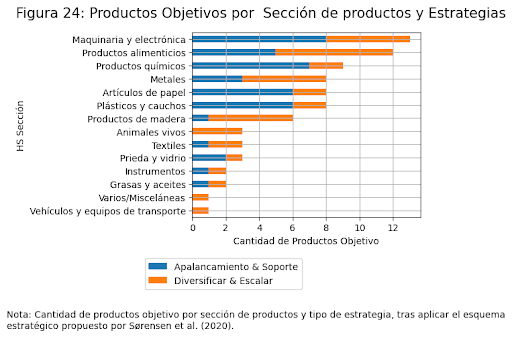
\includegraphics[width=0.9\textwidth]{Figura24.png}
    \end{center}
\end{frame}

% Mercados y Productos Potenciales: Modelo de Gravedad
\begin{frame}{Mercados y Productos Potenciales: Modelo de Gravedad}
    \begin{equation} \tag{17}
    T^{p}_{i,n,t} = exp(\alpha^{p} + \beta^{p}'\ln \phi_{i,n} + \gamma^{p}_{i,t} + \theta^{p}_{n,t}) \cdot \varepsilon^{p}_{i,n,t}
    \end{equation}

    \begin{itemize}
        \item \( \phi_{i,n} \): Accesibilidad bilateral como un vector de medidas de distancia entre el importador \( n \) y el exportador \( i \).
           \item \textbf{El modelo incluye:}
        \begin{itemize}
            \item Variables de la distancia física entre las ciudades más pobladas de los países.
            \item Conjunto de variables indicadoras de contigüidad, vínculos coloniales, si un idioma es hablado por al menos el 9\% de la población en ambos países.
            \item Si dos países son parte del mismo acuerdo comercial regional.
        \end{itemize}
        \item Los términos \( \theta^{p}_{n,t} \) y \( \gamma^{p}_{i,t} \) refieren a los efectos fijos de año-importador y año-exportador respectivamente.
    \end{itemize}
\end{frame}


%Resultados Gravity
\begin{frame}{Mercados y Productos Potenciales: Resultados Gravity}
    \begin{center}
        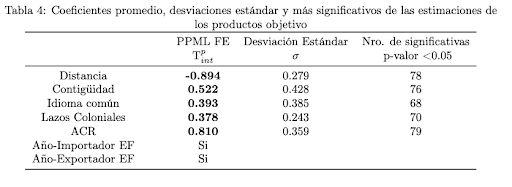
\includegraphics[width=1.1\textwidth]{Tabla4.png}
    \end{center}
        \begin{itemize}
        \footnotesize {Nota: La variable dependiente es el monto de comercio bilateral  en los años 2011-19; los coeficientes se refieren a promedios de 79 regresiones (una para cada producto objetivo); desviaciones estándar del conjunto de parámetros para cada variable; cantidad de coeficientes estimados significativos.} 
    \end{itemize}
\end{frame}

% Mercados y Productos potenciales: Medidas de Potencialidad
\begin{frame}{Mercados y Productos potenciales: Medidas de Potencialidad}
    \begin{itemize}
        \item \textbf{Estimación de flujo de comercio a partir de modelo de gravedad:}
    \end{itemize}
    \begin{equation} \tag{18}
    \hat{T}^{p}_{ECU,n,t} = \exp(\hat{\alpha}^{p} + \hat{\beta}^{p}'\ln \phi_{ECU,n} + \hat{\theta}^{p}_{n,t})
    \end{equation}
    \begin{itemize}
        \item Los coeficientes \( \hat{\alpha} \), \( \hat{\beta} \) y \( \hat{\theta} \) son los valores estimados del modelo de regresión PPML con efectos fijos en los años exportador e importador.
        \item El enfoque de la ecuación 18 busca evitar posibles distorsiones en la capacidad actual de exportación de Ecuador para los productos objetivo.
    \end{itemize}
\end{frame}

% Nueva diapositiva: Medidas de Potencialidad
\begin{frame}{Mercados y Productos potenciales: Medidas de Potencialidad}
    \begin{itemize}
        \item \textbf{Potencial de productos:} Permite calcular el comercio potencial total de cada producto objetivo entre Ecuador y el resto de países.
    \end{itemize}
    \vspace{0.2cm}
    \begin{equation}
    PEP_{n} = \sum_{c,t} \hat{T}^p_{Ecu, n, t}
    \end{equation}

    \vspace{0.5cm}

    \begin{itemize}
        \item \textbf{Potencial de mercados:} Permite capturar el valor de exportación total estimado de todos los productos objetivo de Ecuador a cada país \( n \) durante un período de nueve años (2011-2019).
    \end{itemize}
    \vspace{0.2cm}
    \begin{equation}
    MEP_{n} = \sum_{p,t} \hat{T}^p_{Ecu, n, t}
    \end{equation}
\end{frame}


% Mercados y Productos potenciales: PEP

\begin{frame}{Mercados y Productos potenciales: Medidas de Potencialidad}
    \begin{center}
        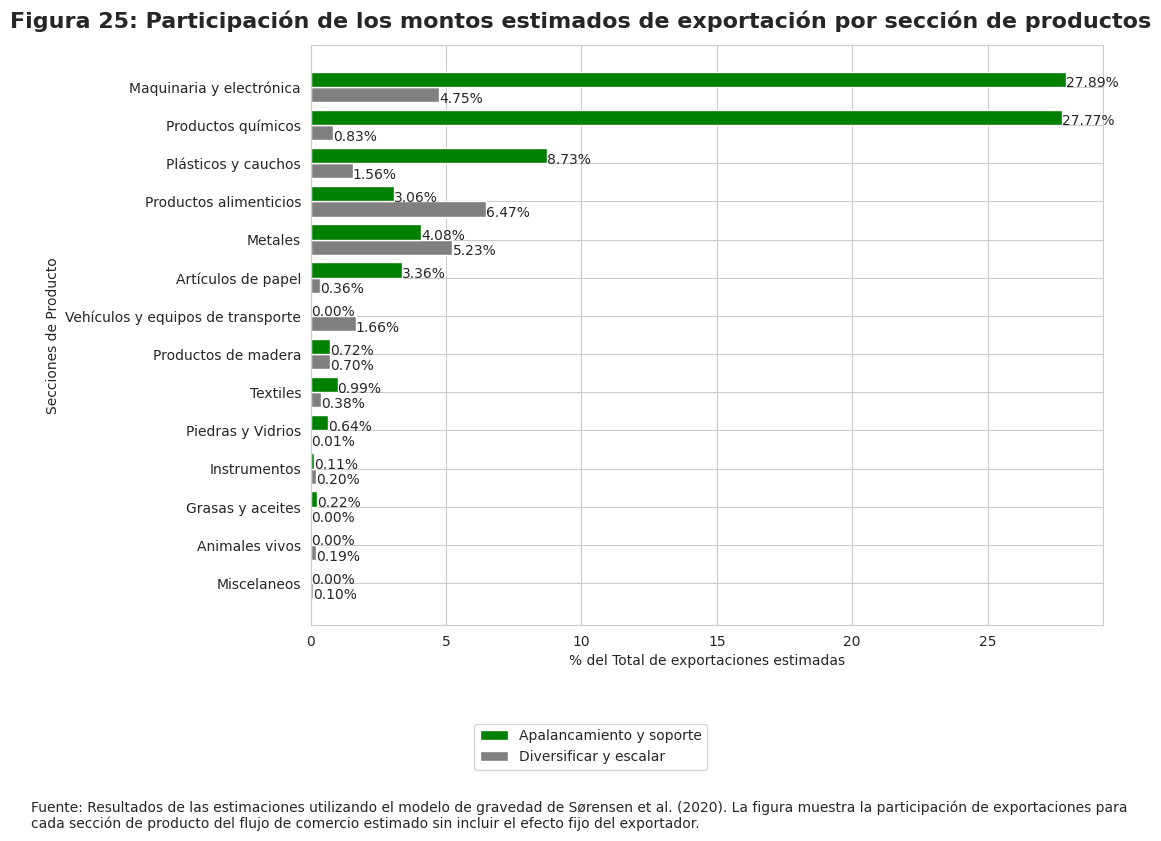
\includegraphics[width=0.9\textwidth]{Figura25.png}
    \end{center}
\end{frame}


% Modelo de Gravedad
\begin{frame}{Modelo de Gravedad}
    \begin{itemize}
        \item Estimación de flujos comerciales entre países.
        \item Incluye variables como distancia física, vínculos coloniales y acuerdos comerciales.
        \item Resultados permiten identificar mercados potenciales para productos ecuatorianos.
    \end{itemize}
\end{frame}

% Productos Potenciales por Tipos de sección
\begin{frame}{Productos Potenciales por Tipos de sección}
    \begin{table}[h]
    \centering
    \vspace{-0.2cm}{Tabla 6: Flujo de comercio estimado de las seis secciones de productos sobre los mercados potenciales (valores en dólares)}
    \begin{adjustbox}{width=0.9\textwidth,margin=0.1cm}
    \begin{tabular}{ l c c  c }
    \hline
    \\
    Sección de productos  &{$PEP^{p}_{nt} $ (\text{USD})} &  {$PEP^{p}_{nt} avg $(\text{USD})} & {${PEP}^{p}_{nt} avg /PIB_{2019}(\%)$} \\
    &(1)&(2) &(3) \\
    \hline
    \\
    Maquinaria y electrónica &82659.79 & 9184.42 & 8.54\\
    Productos químicos &71832.54 &  7981.39 & 7.42\\
    Plásticos y cauchos &26061.12 & 2895.68 & 2.69 \\
    Metales  & 24002.58 &2666.95 &2.48\\
    Productos alimenticios & 22806.64 & 2534.07 & 2.36 \\
    Artículos de papel & 9539.02 & 1059.89 & 0.99\\
    \\
    \hline
    \end{tabular}
    \end{adjustbox}
    \vspace{0.2cm}

      \tiny{ Montos USD \$ en millones, los flujos de comercio promedio son por nueve años (2011-2019), los países considerados son los que tienen mayor potencial de exportación y que refieren a los ilustrados en el primer y cuarto cuadrante de la Figura 23. El valor del PIB de Ecuador corresponde al año 2019 (en US\$ a precios actuales) y se obtuvo del repositorio de datos del Banco Mundial (2023) }
    \end{table}
\end{frame}

% Mercados y Productos potenciales: MEP

\begin{frame}{Mercados y Productos potenciales: Medidas de Potencialidad}
    \begin{center}
        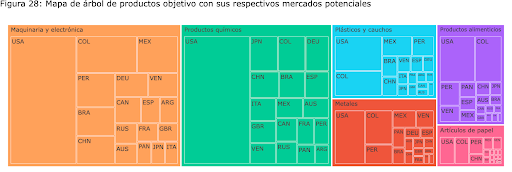
\includegraphics[width=1.05\textwidth]{Figura28.png}
    \end{center}
\end{frame}

% Conclusiones
\begin{frame}{Conclusiones}
    \begin{itemize}
        \item El país enfrenta dificultades para diversificar y sofisticar su economía.
        \item Es necesario priorizar sectores con mayor complejidad económica y valor agregado.
        \item Sectores prometedores: maquinarias, electrónica y productos químicos.
    \end{itemize}
\end{frame}
% Diapositivas adicionales
\begin{frame}
    \vfill
    \begin{center}
        \textbf{Diapositivas adicionales}
    \end{center}
    \vfill
\end{frame}
%Estrategias de Selección: Interpretación estratégica

\begin{frame}{Estrategias de Selección: Interpretación estratégica}
    \begin{center}
        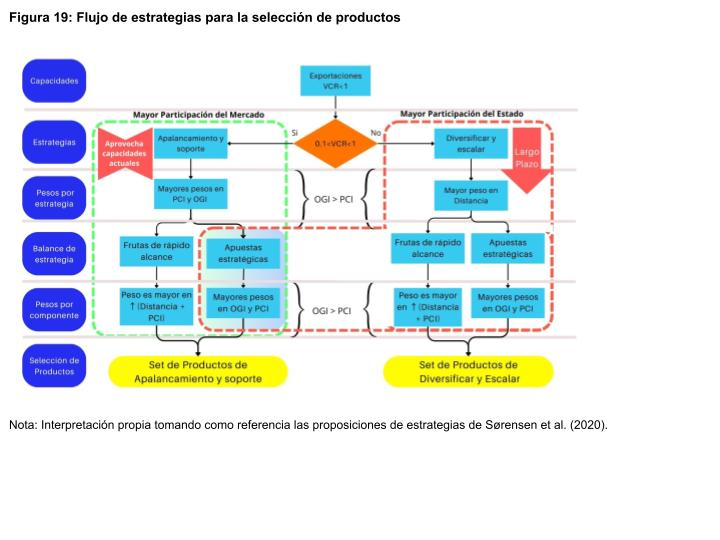
\includegraphics[width=1.1\textwidth]{Figura19.jpg}
    \end{center}
    \vspace{-0.25cm}

\end{frame}

% Estrategias de Selección: Criterios de Asignación de pesos
\begin{frame}{Estrategias de Selección: Criterios de Asignación de pesos}
    \begin{table}[!ht]
    \centering
    \begin{adjustbox}{max width=1.05\textwidth} % Ajustar tamaño de la tabla

    \begin{tabular}{ll}
    \multicolumn{2}{l}{\textbf{Tabla 2: Criterios de asignación de pesos}} \\
    \hline
    \\
    \textbf{Criterio 1:} & \\
    & \textbf{Apalancamiento \& Soporte:} Distancia tiene menor peso con respecto a la suma de pesos de PCI y OGI. \\
    & \textbf{Diversificar \& escalar:} Distancia tiene un peso mayor o igual con respecto a la suma de puntajes de PCI y OGI. \\
    \\
    \textbf{Criterio 2:} & \\
    & \textbf{Frutas de rápido alcance:} La suma de pesos de PCI y Distancia debe superar a la de OGI. \\
    \\
    \textbf{Criterio 3:} & \\
    & El peso de OGI debe siempre ser mayor a PCI en todos los componentes y estrategias. \\
    \\
    \hline
    \multicolumn{2}{l}{\textit{Fuente:} Elaboración propia tomando como referencias las Proposiciones de Sørensen et al. (2020)} \\
    \end{tabular}
    \end{adjustbox}
    \end{table}
\end{frame}


% Estrategias de Selección: Definición de Estrategias (1)
\begin{frame}{Estrategias de Selección: Definición de Estrategias (1)}
    \begin{table}[!ht]
    \centering
    \vspace{-0.2cm}{Tabla A1: Efecto de la distancia y exportaciones en la aparición de producto}
    \begin{adjustbox}{width=0.9\textwidth,margin=0.9cm}

    \begin{tabular}{lrrrr}
        \toprule
        & (1) & (2) & (3) & (4)\\ 
        \midrule
        Distancia (2015) & -0.030*** & -0.031*** & -0.009*** & -0.010*** \\
        & (0.001) & (0.001) & (0.002) & (0.001) \\
        $D^{export}$(2015) & 0.026*** & 0.025*** & 0.020*** & 0.020*** \\
        & (0.001) & (0.001) & (0.002) & (0.002) \\
        Distancia $\times D^{export}$(2015) & & 0.002** & & 0.002** \\
        & & (0.001) & & (0.002) \\
        \midrule
        Año EF & Si & Si & Si & Si \\
        País EF & Si & Si & Si & Si \\
        Observaciones & 532,316 & 532,316 & 43,240 & 43,240 \\
        R-squared & 0.018 & 0.018 & 0.013 & 0.013 \\
        \bottomrule
    \end{tabular}
    \end{adjustbox}

    \vspace{0.2cm}
    \tiny{Fuente: Réplica y adaptación de la proposición 1 del trabajo de Sørensen et al.(2020). Errores estándar robustos entre paréntesis. *** p\textless0.01, ** p\textless0.05, * p\textless0.1. La columna 1 y 2 refieren a los coeficientes y errores estándar sobre todos los países de la base. La columna 3 y 4 refieren a los coeficientes errores estándar sobre los países de la región. Los países incluyen: Brasil, Colombia, Bolivia, Paraguay, Perú, Chile, Argentina, Uruguay y Venezuela.}
    \end{table}
\end{frame}
% Estrategias de Selección: Definición de Estrategias (2)
\begin{frame}{Estrategias de Selección: Definición de Estrategias (2)}
    \begin{center}
        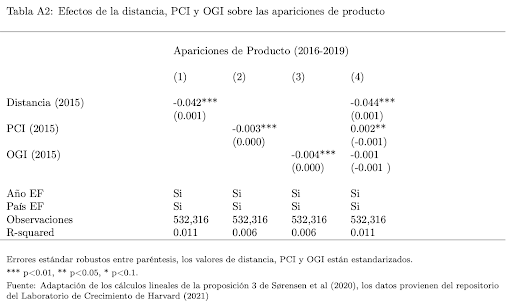
\includegraphics[width=1.0\textwidth]{TablaA2.png}
    \end{center}
    \vspace{-0.25cm}

\end{frame}

% Mercados y Productos Potenciales: Total de secciones de productos identificados
\begin{frame}{Mercados y Productos Potenciales: Total de secciones de productos identificados}
    \begin{table}[!ht]
    \centering
    \vspace{-0.2cm}\tiny{Tabla 5: Montos y \% con respecto al PIB de los flujos de comercio estimados para los catorce secciones de productos.}
    \begin{adjustbox}{width=0.9\textwidth,margin=0.9cm}
    \begin{tabular}{lcccccc}
    \hline
    \\
    Sección de productos & {${PEP}^{p}_{nt}$  (\text{USD})} & {${PEP}^{p}_{nt} avg $ (\text{USD})} &
    {${PEP}^{p}_{nt} avg /PIB_{2019}(\%)$} \\
    &(1)&(2)&(3) \\
    \hline
    \\
    Maquinaria y electrónica  & 108441.25 & 12049.03 & 11.20 \\
    Productos Químicos & 95012.59 & 10556.95   & 9.81 \\
    Plásticos y cauchos & 34172.67 & 3796.96 & 3.53 \\
    Productos alimenticios & 31638.92 & 3515.44   & 3.27 \\
    Metales & 30947.58 & 3438.62  & 3.20 \\
    Artículos de papel & 12366.00 & 1374.00 &  1.28 \\
    Vehículos y equipos de transporte & 5528.82 & 614.31 & 0.57\\
    Productos de madera & 4716.04 & 524.00 &   0.49 \\
    Textiles & 4555.12 & 506.12 & 0.47 \\
    Piedra y vidrio & 2162.83 & 240.31 &   0.22 \\
    Instrumentos & 1035.71 & 115.08 &   0.11 \\
    Grasas y Aceites & 417.96 & 80.95 &  0.08 \\
    Animales vivos & 641.75 & 71.31 & 0.07 \\
    Misceláneos & 329.35 & 36.59 &   0.03 \\
    \\
    \hline
    \end{tabular}
    \end{adjustbox}
    \vspace{0.2cm}
    \tiny{Montos en USD\$ y en millones, el flujo de comercio promedio es por nueve años (2011-2019), el valor del PIB de Ecuador corresponde al año 2019 (en US\$ a precios actuales) y se obtuvo del repositorio de datos del Banco Mundial (2023).}
    \end{table}
\end{frame}
\end{document}
